\documentclass[10pt]{beamer}
\usepackage[utf8]{inputenc}
\usepackage[francais]{babel}
\usepackage[T1]{fontenc}
\usepackage[export]{adjustbox}
\newcommand\Fontvi{\fontsize{8}{7.2}\selectfont}
\usepackage{tabularx}
\usepackage{minted}
\usemintedstyle{colorful}
\definecolor{mygray}{gray}{0.95}
\newenvironment{code}{\captionsetup{type=listing}}{}

\usepackage{hyperref}
% \hypersetup{
%     colorlinks,
%     citecolor=black,
%     filecolor=black,
%     linkcolor=black,
%     urlcolor=blue
% }
\usepackage{graphicx}
\usepackage{multimedia}
% \usepackage[table]{xcolor}

\usetheme{Frankfurt}
\usecolortheme{default}

\addtobeamertemplate{navigation symbols}{}{%
    \usebeamerfont{footline}%
    \usebeamercolor[fg]{footline}%
    \hspace{1em}%
    \insertframenumber/\inserttotalframenumber
}

\titlegraphic{
\includegraphics[width=0.5\textwidth]{images/title.png}}

\begin{document}
\logo{%
    \makebox[0.95\paperwidth]{%
        
\includegraphics[width=2.5cm,keepaspectratio]{images/hepia.jpg}%
        \hfill%
        
\includegraphics[width=2.5cm,keepaspectratio]{images/hesso.jpg}%
    }%
}

\title{TagFS - Système d'étiquetage des fichiers avec Rust}
\author{Steven Liatti}
\institute{Projet de bachelor - Prof. Florent Glück - Hepia ITI 3\up{ème} année}
\date{4 septembre 2018}

\begin{frame}
\titlepage
\end{frame}

\begin{frame}
    \frametitle{Plan}
    \setcounter{tocdepth}{1}
    \tableofcontents
\end{frame}

%%%%%%%%%%%%%%%%%%%%%%%%%%%%%%%%%%%%%%%%%%%%%%%%%%%%%%%%%%%%%%%%%%%%%%%%%%%%%%%%%%%%%%%%%%%%%%%%%%%
%%%%%%%%%%%%%%%%%%%%%%%%%%%%%%%%%%%%%%%%%%%%%%%%%%%%%%%%%%%%%%%%%%%%%%%%%%%%%%%%%%%%%%%%%%%%%%%%%%%
\section{Introduction}
\subsection{Problématiques}
\begin{frame}
    \frametitle{\subsecname}
    \begin{itemize}
        \item Nombre de fichiers énorme.
        \pause
        \item Difficulté à retrouver des fichiers.
        \pause
        \item Plusieurs emplacements logiques pour un seul fichier.
        \pause
    \end{itemize}
    \Large\textbf{Système de "tagging" de fichiers et répertoires avec possibilité de recherche par tags.}
\end{frame}

\subsection{Cahier des charges}
\begin{frame}
    \frametitle{\subsecname}
    \begin{itemize}
        \item Répertorier les applications existantes permettant d'étiqueter les fichiers.
        \pause
        \item Étudier une façon de stocker les tags avec les fichiers : les attributs étendus des fichiers (XATTR).
        \pause
        \item Analyser les moyens d'indexer et de surveiller une arborescence de fichiers.
        \pause
        \item Concevoir et implémenter le système (open source et sur Linux) et mesurer ses performances.
        \pause
        \item Étudier et s'approprier le langage Rust.
    \end{itemize}
\end{frame}

%%%%%%%%%%%%%%%%%%%%%%%%%%%%%%%%%%%%%%%%%%%%%%%%%%%%%%%%%%%%%%%%%%%%%%%%%%%%%%%%%%%%%%%%%%%%%%%%%%%
%%%%%%%%%%%%%%%%%%%%%%%%%%%%%%%%%%%%%%%%%%%%%%%%%%%%%%%%%%%%%%%%%%%%%%%%%%%%%%%%%%%%%%%%%%%%%%%%%%%
\section{Solutions existantes}
\subsection{TMSU, Tagsistant et TagSpaces}
\begin{frame}
    \frametitle{\subsecname}
    \begin{columns}[T]
        \begin{column}{.35\textwidth}
        \fontsize{7pt}{8}\selectfont
            \begin{center}
                \begin{itemize}
                    \item Gestion des tags.
                    \item Liste de fichiers liés aux tags.
                    \item CLI ou GUI.
                \end{itemize}
                \pause[3]
                \bigbreak
                \begin{tabularx}{4.5cm}{|p{1.8cm}|X|} \hline
                    \textbf{Points positifs} & \textbf{Points négatifs} \\ \hline
                    Simples & Dépendance à une BDD externe \\ \hline
                    Rapides et efficaces & Modification et accès uniquement par l'app \\ \hline
                    Open source & \\ \hline
                \end{tabularx}
            \end{center}
        \end{column}
        \pause[2]
        \begin{column}{.65\textwidth}
            \begin{flushright}
                \begin{figure}
                    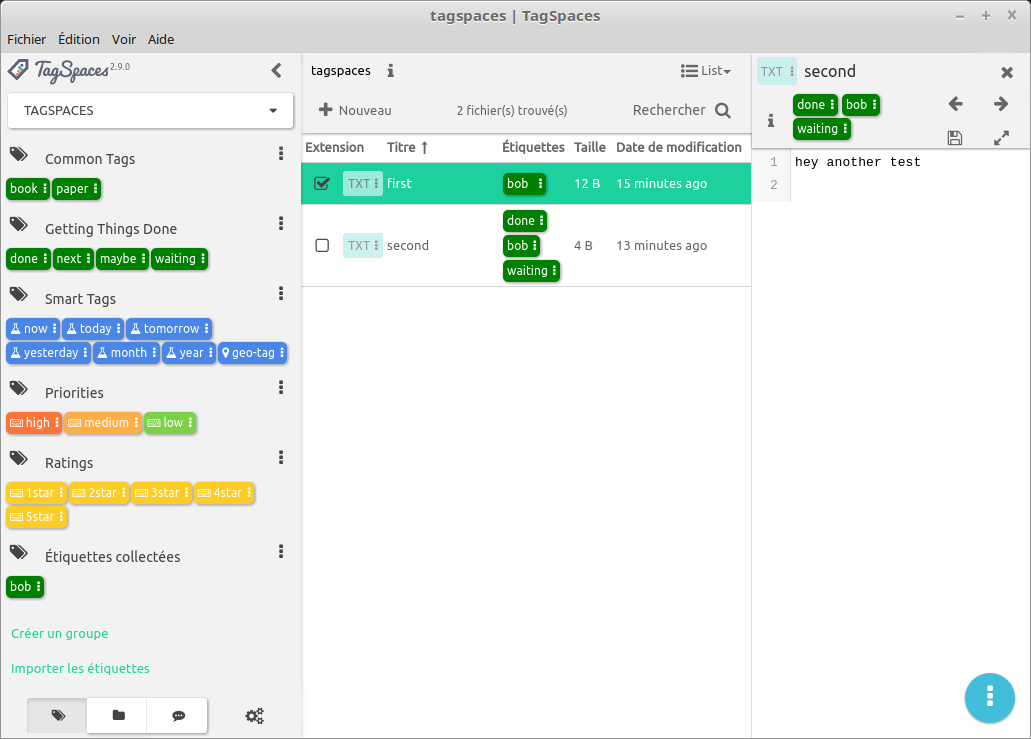
\includegraphics[width=0.98\textwidth]{images/tagspaces.png}
                    \caption{Utilisation de TagSpaces}
                \end{figure}
            \end{flushright}
        \end{column}
    \end{columns}
\end{frame}

\subsection{macOS}
\begin{frame}
    \frametitle{\subsecname}
    \fontsize{6pt}{8}\selectfont
    \begin{columns}[T]
        \begin{column}{.65\textwidth}
            \begin{center}
                \begin{figure}
                    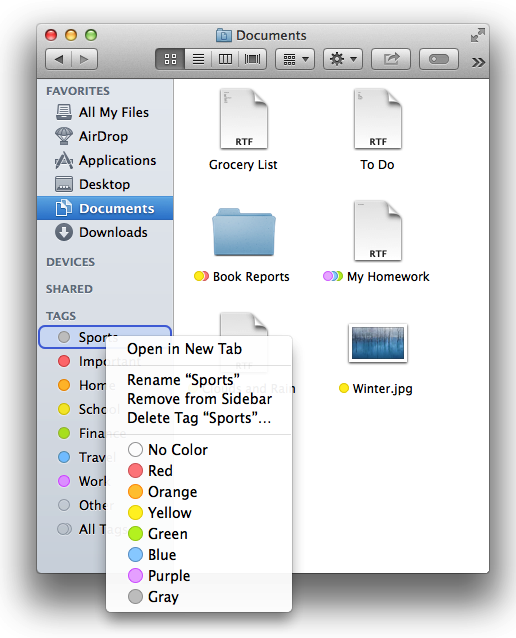
\includegraphics[width=0.6\textwidth]{images/macos_tags.png}
                    \caption{Gestion d'un tag dans le Finder - Apple}
                \end{figure}
            \end{center}
        \end{column}
        \pause
        \fontsize{8pt}{9}\selectfont
        \begin{column}{.35\textwidth}
            \begin{center}
                \begin{tabularx}{3.5cm}{|X|X|} \hline
                    \textbf{Points positifs} & \textbf{Points négatifs} \\ \hline
                    Système de tags intégré à l'explorateur de fichiers & Code propriétaire \\ \hline
                    Stocke les tags dans les XATTR & Seulement pour macOS \\ \hline
                    Performant & \\ \hline
                \end{tabularx}
            \end{center}
        \end{column}
    \end{columns}
\end{frame}

%%%%%%%%%%%%%%%%%%%%%%%%%%%%%%%%%%%%%%%%%%%%%%%%%%%%%%%%%%%%%%%%%%%%%%%%%%%%%%%%%%%%%%%%%%%%%%%%%%
%%%%%%%%%%%%%%%%%%%%%%%%%%%%%%%%%%%%%%%%%%%%%%%%%%%%%%%%%%%%%%%%%%%%%%%%%%%%%%%%%%%%%%%%%%%%%%%%%%
\section{Architecture}
\subsection{Gestion des tags}
\begin{frame}
    \frametitle{\subsecname}
    \begin{itemize}
        \pause
        \item Stockage des tags avec les fichiers (indépendance à une base de données).
        \pause
        \item Outil dédié de gestion de tags (confort d'utilisation).
    \end{itemize}
\end{frame}

\subsection{Indexation des fichiers et des tags}
\begin{frame}
    \frametitle{\subsecname}
    \begin{columns}[T]
        \pause
        \begin{column}{.6\textwidth}
            \begin{figure}
                \begin{center}
                    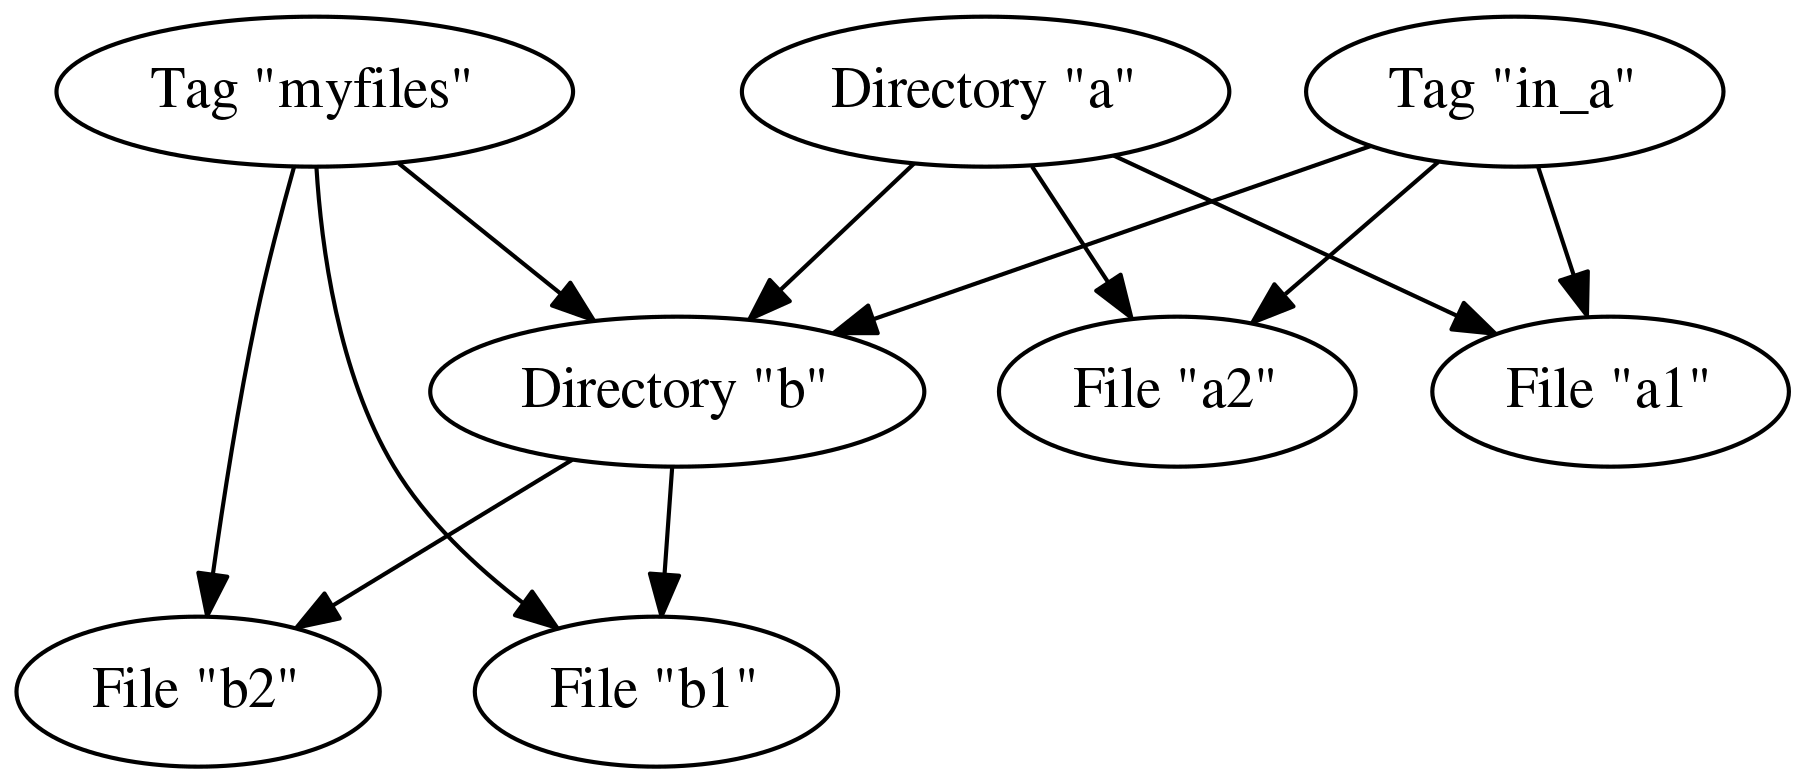
\includegraphics[width=1\textwidth]{images/graph.png}
                    \caption{Graphe de tags, fichiers et répertoires}
                \end{center}
            \end{figure}
        \end{column}
        \pause
        \begin{column}{.4\textwidth}
            \begin{figure}
                \begin{center}
                    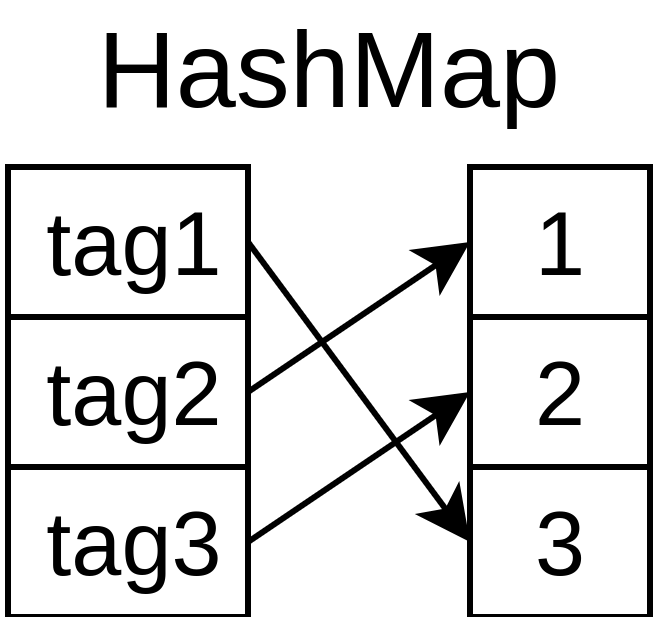
\includegraphics[width=0.5\textwidth]{images/hashmap.png}
                    \caption{HashMap associant le nom du tag à son noeud}
                \end{center}
            \end{figure}
        \end{column}
    \end{columns}
\end{frame}

\subsection{Surveillance du système de fichiers}
\begin{frame}
    \frametitle{\subsecname}
    Mise à jour du graphe lors des événements suivants :
    \bigbreak
    \pause
    \begin{itemize}
        \item Changement sur les tags.
        \pause
        \item Création de fichiers/répertoires.
        \pause
        \item Suppression de fichiers/répertoires.
        \pause
        \item Déplacement/renommage de fichiers/répertoires.
    \end{itemize}
\end{frame}

\subsection{Requêtes de tags et fichiers}
\begin{frame}
    \frametitle{\subsecname}
    \begin{itemize}
        \pause
        \item Lister les fichiers et répertoires associés à des tags => requêtes sous forme 
            d'expressions logiques (opérateurs logiques).
        \pause
        \item Lister les tags existants.
        \pause
        \item Renommer un tag.
    \end{itemize}
\end{frame}

%%%%%%%%%%%%%%%%%%%%%%%%%%%%%%%%%%%%%%%%%%%%%%%%%%%%%%%%%%%%%%%%%%%%%%%%%%%%%%%%%%%%%%%%%%%%%%%%%%%
%%%%%%%%%%%%%%%%%%%%%%%%%%%%%%%%%%%%%%%%%%%%%%%%%%%%%%%%%%%%%%%%%%%%%%%%%%%%%%%%%%%%%%%%%%%%%%%%%%%
\section{Technologies}
\subsection{Rust}
\begin{frame}
    \frametitle{\subsecname}
    \begin{itemize}
        \item Langage système moderne, performant, fiable (plus sécurisé qu'Ada), compilé, et fortement typé.
        \pause
        \item Disponible sur Linux, Windows et macOS.
        \pause
        \item Cargo : outil de compilation et d'exécution et gestionnaire de paquets intégré à Rust.
        \pause
        \item Structures, collections, généricité, immutabilité, énumérations et \textit{pattern matching}.
        \pause
        \item Gestion des erreurs et tests unitaires.
        \pause
        \item \textbf{\textit{Ownership}, \textit{Borrowing} (références)}.
    \end{itemize}
\end{frame}

\subsection{Attributs étendus (XATTR)}
\begin{frame}
    \frametitle{\subsecname}
    \begin{itemize}
        \pause
        \item Métadonnées sous forme de paires \mintinline{text}{nom:valeur}.
        \pause
        \item Nom = chaine de caractères, valeur = chaine de caractères ou données binaires.
        \pause
        \item Existent sous ext2-3-4, XFS, Btrfs, UFS1-2, NTFS, HFS+, ZFS.
        \pause
        \item Outils CLI pour facilement les manipuler.
    \end{itemize}
\end{frame}

\subsection{Inotify}
\begin{frame}
    \frametitle{\subsecname}
    \begin{itemize}
        \pause
        \item API de notifications d'événements sur le système de fichiers.
        \pause
        \item Trois appels système : initialisation, ajout de surveillance sur un chemin de fichiers 
            donné et suppression de cette surveillance.
        \pause
        \item Lecture d'un événement avec read().
    \end{itemize}
\end{frame}

% \subsection{Sockets}
% \begin{frame}
%     \frametitle{\subsecname}
%     \begin{figure}
%         \begin{center}
%             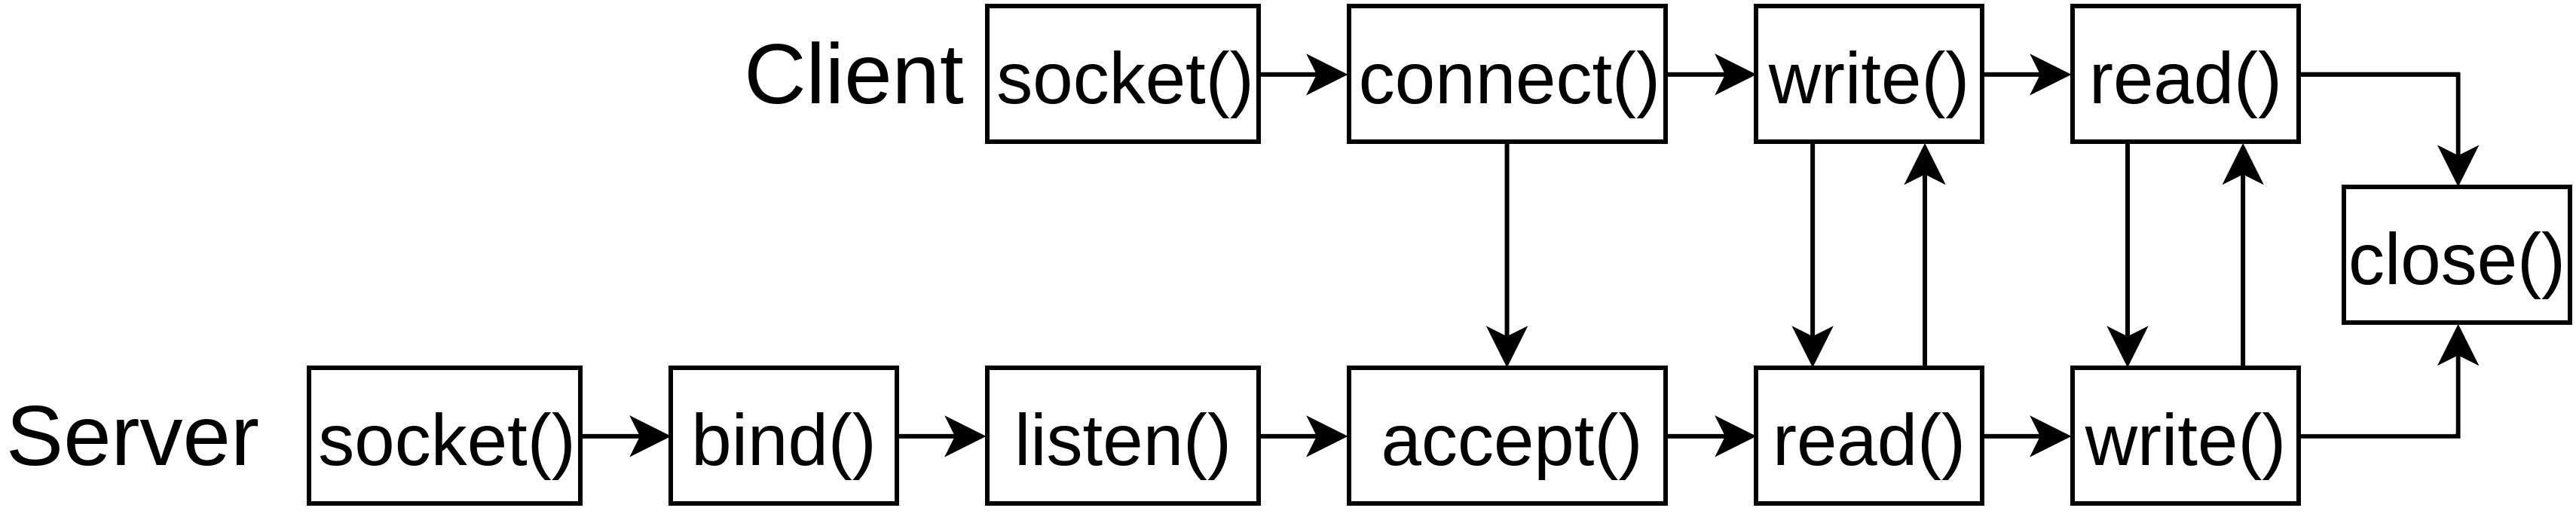
\includegraphics[width=1\textwidth]{images/sockets2.png}
%         \end{center}
%     \end{figure}
% \end{frame}

%%%%%%%%%%%%%%%%%%%%%%%%%%%%%%%%%%%%%%%%%%%%%%%%%%%%%%%%%%%%%%%%%%%%%%%%%%%%%%%%%%%%%%%%%%%%%%%%%%%
%%%%%%%%%%%%%%%%%%%%%%%%%%%%%%%%%%%%%%%%%%%%%%%%%%%%%%%%%%%%%%%%%%%%%%%%%%%%%%%%%%%%%%%%%%%%%%%%%%%
\section{Réalisation}
\subsection{Tag Manager}
\begin{frame}
    \frametitle{\subsecname}
    \begin{figure}
        \begin{center}
            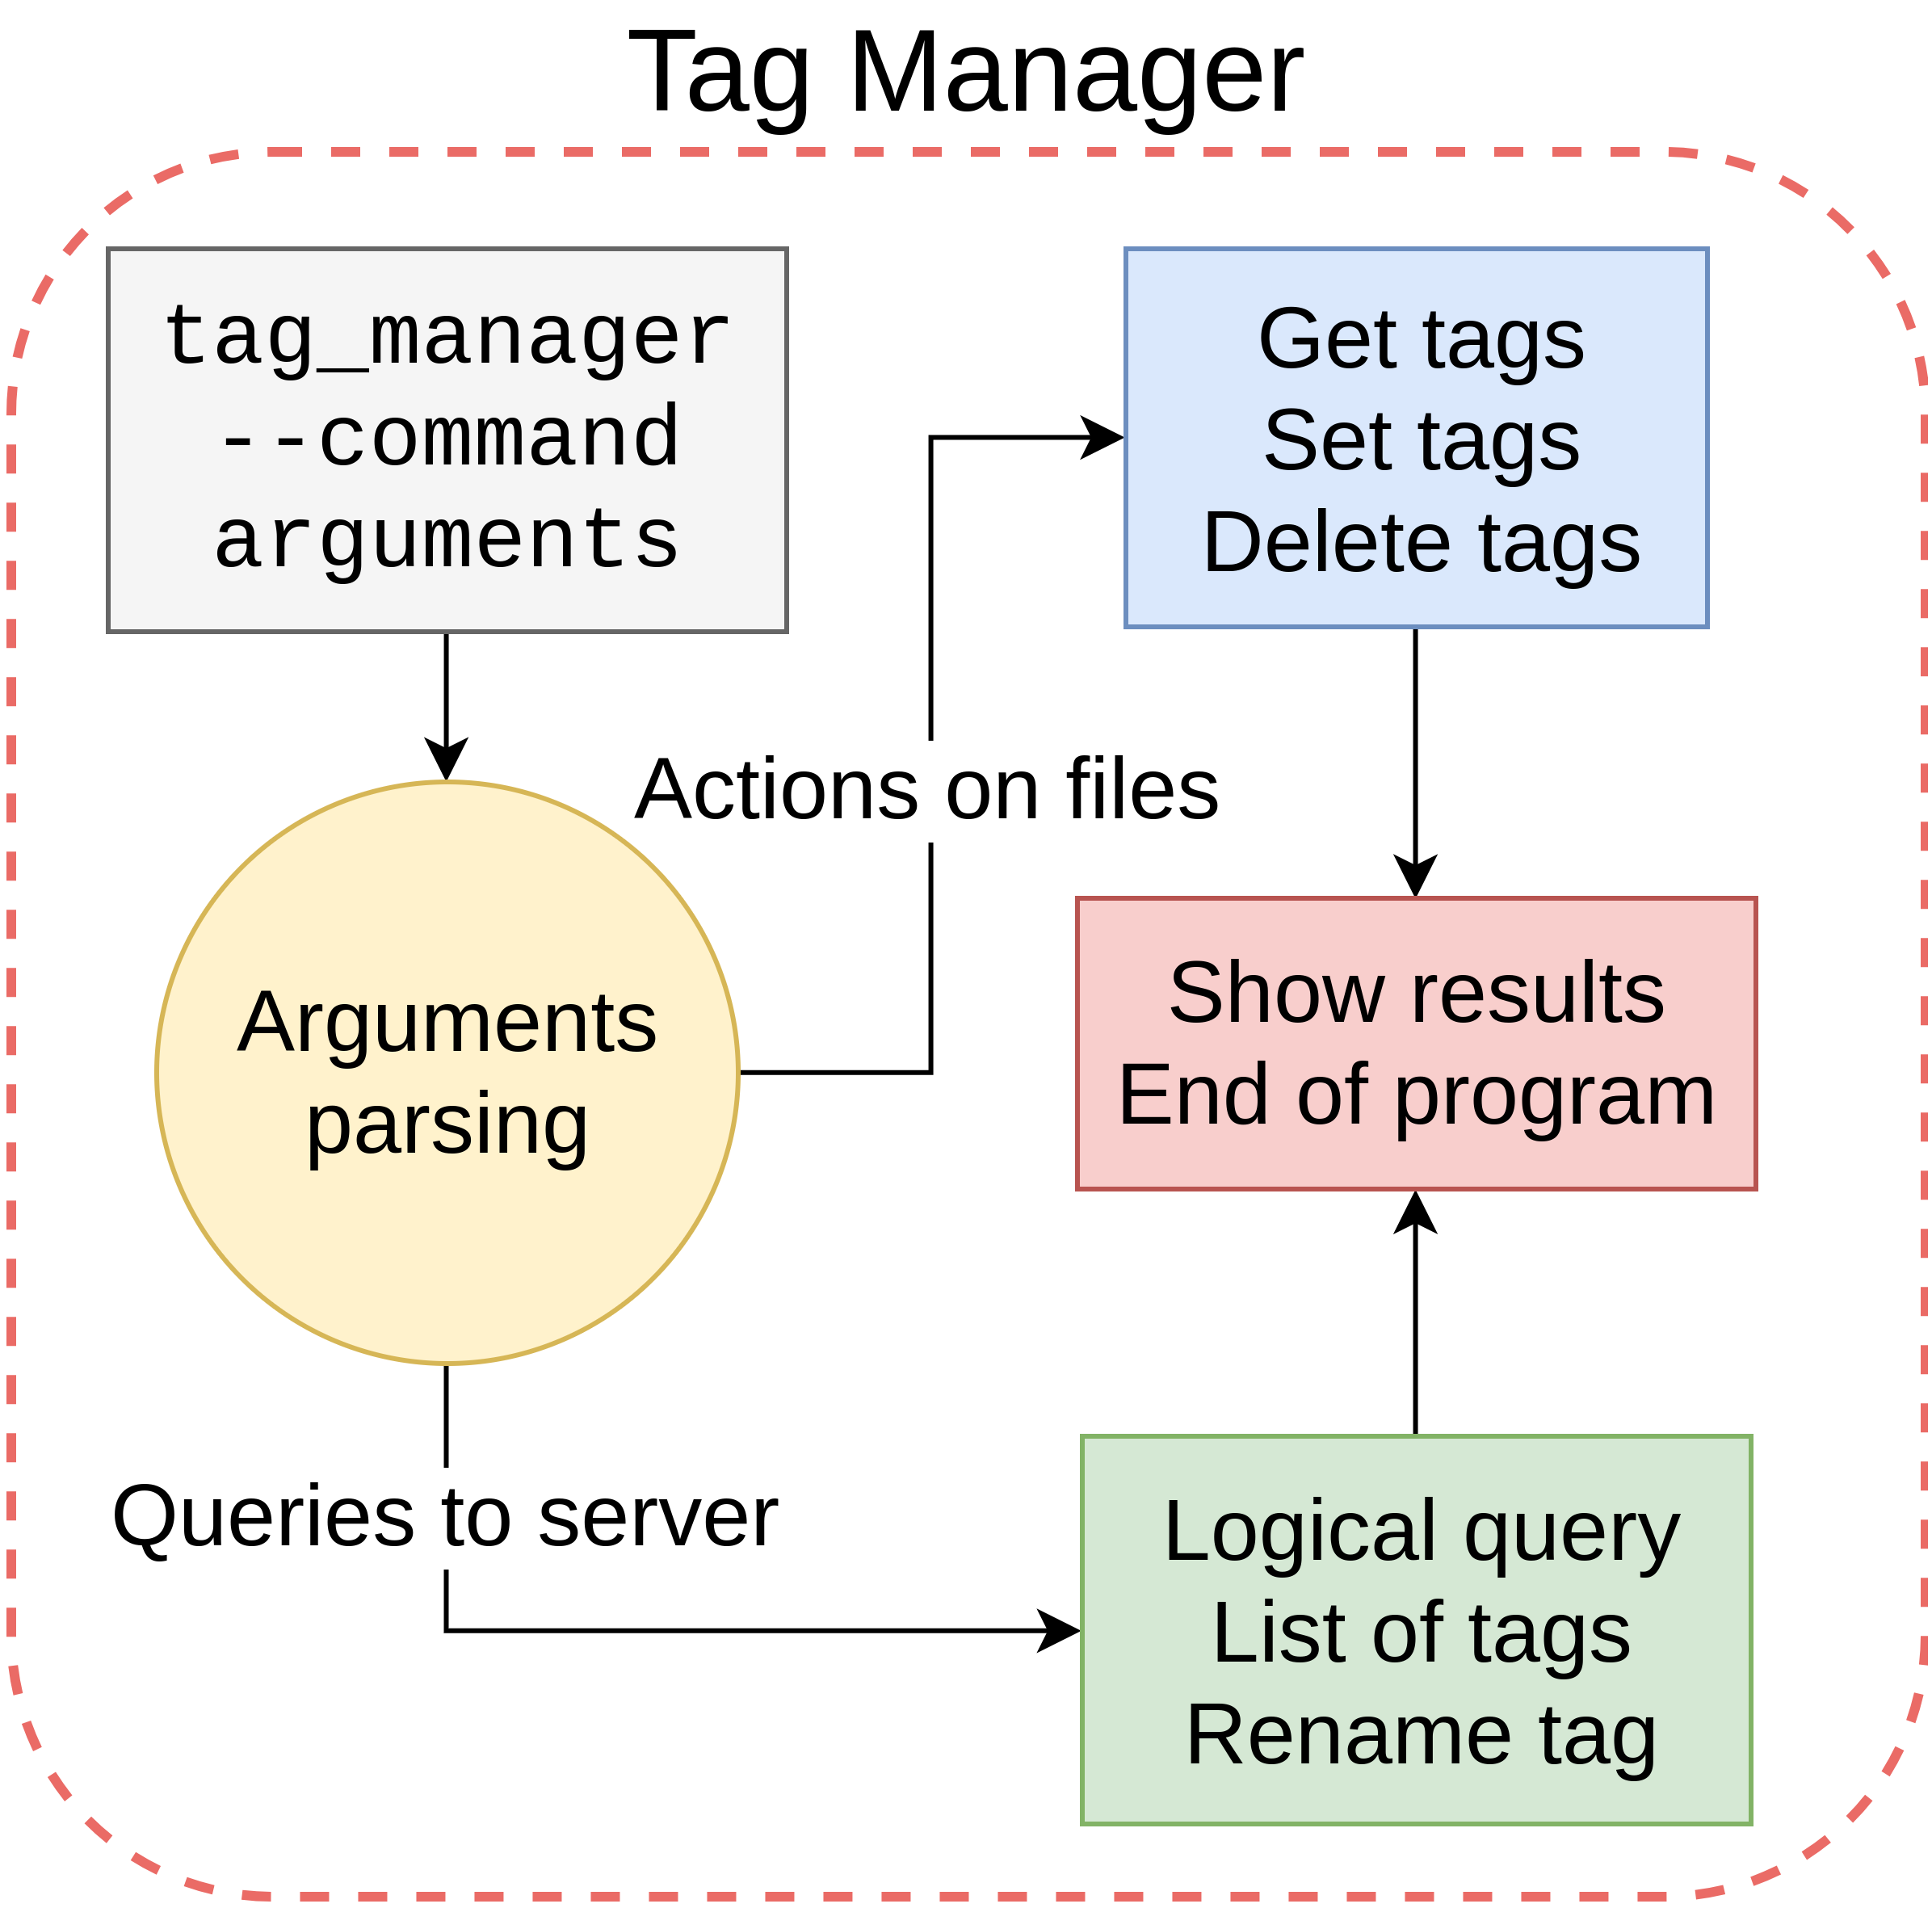
\includegraphics[width=0.6\textwidth]{images/tag_manager2.png}
            \caption{Fonctionnement de Tag Manager}
        \end{center}
    \end{figure}
\end{frame}

\subsection{Tag Engine}
\begin{frame}
    \frametitle{\subsecname}
    \begin{figure}
        \begin{center}
            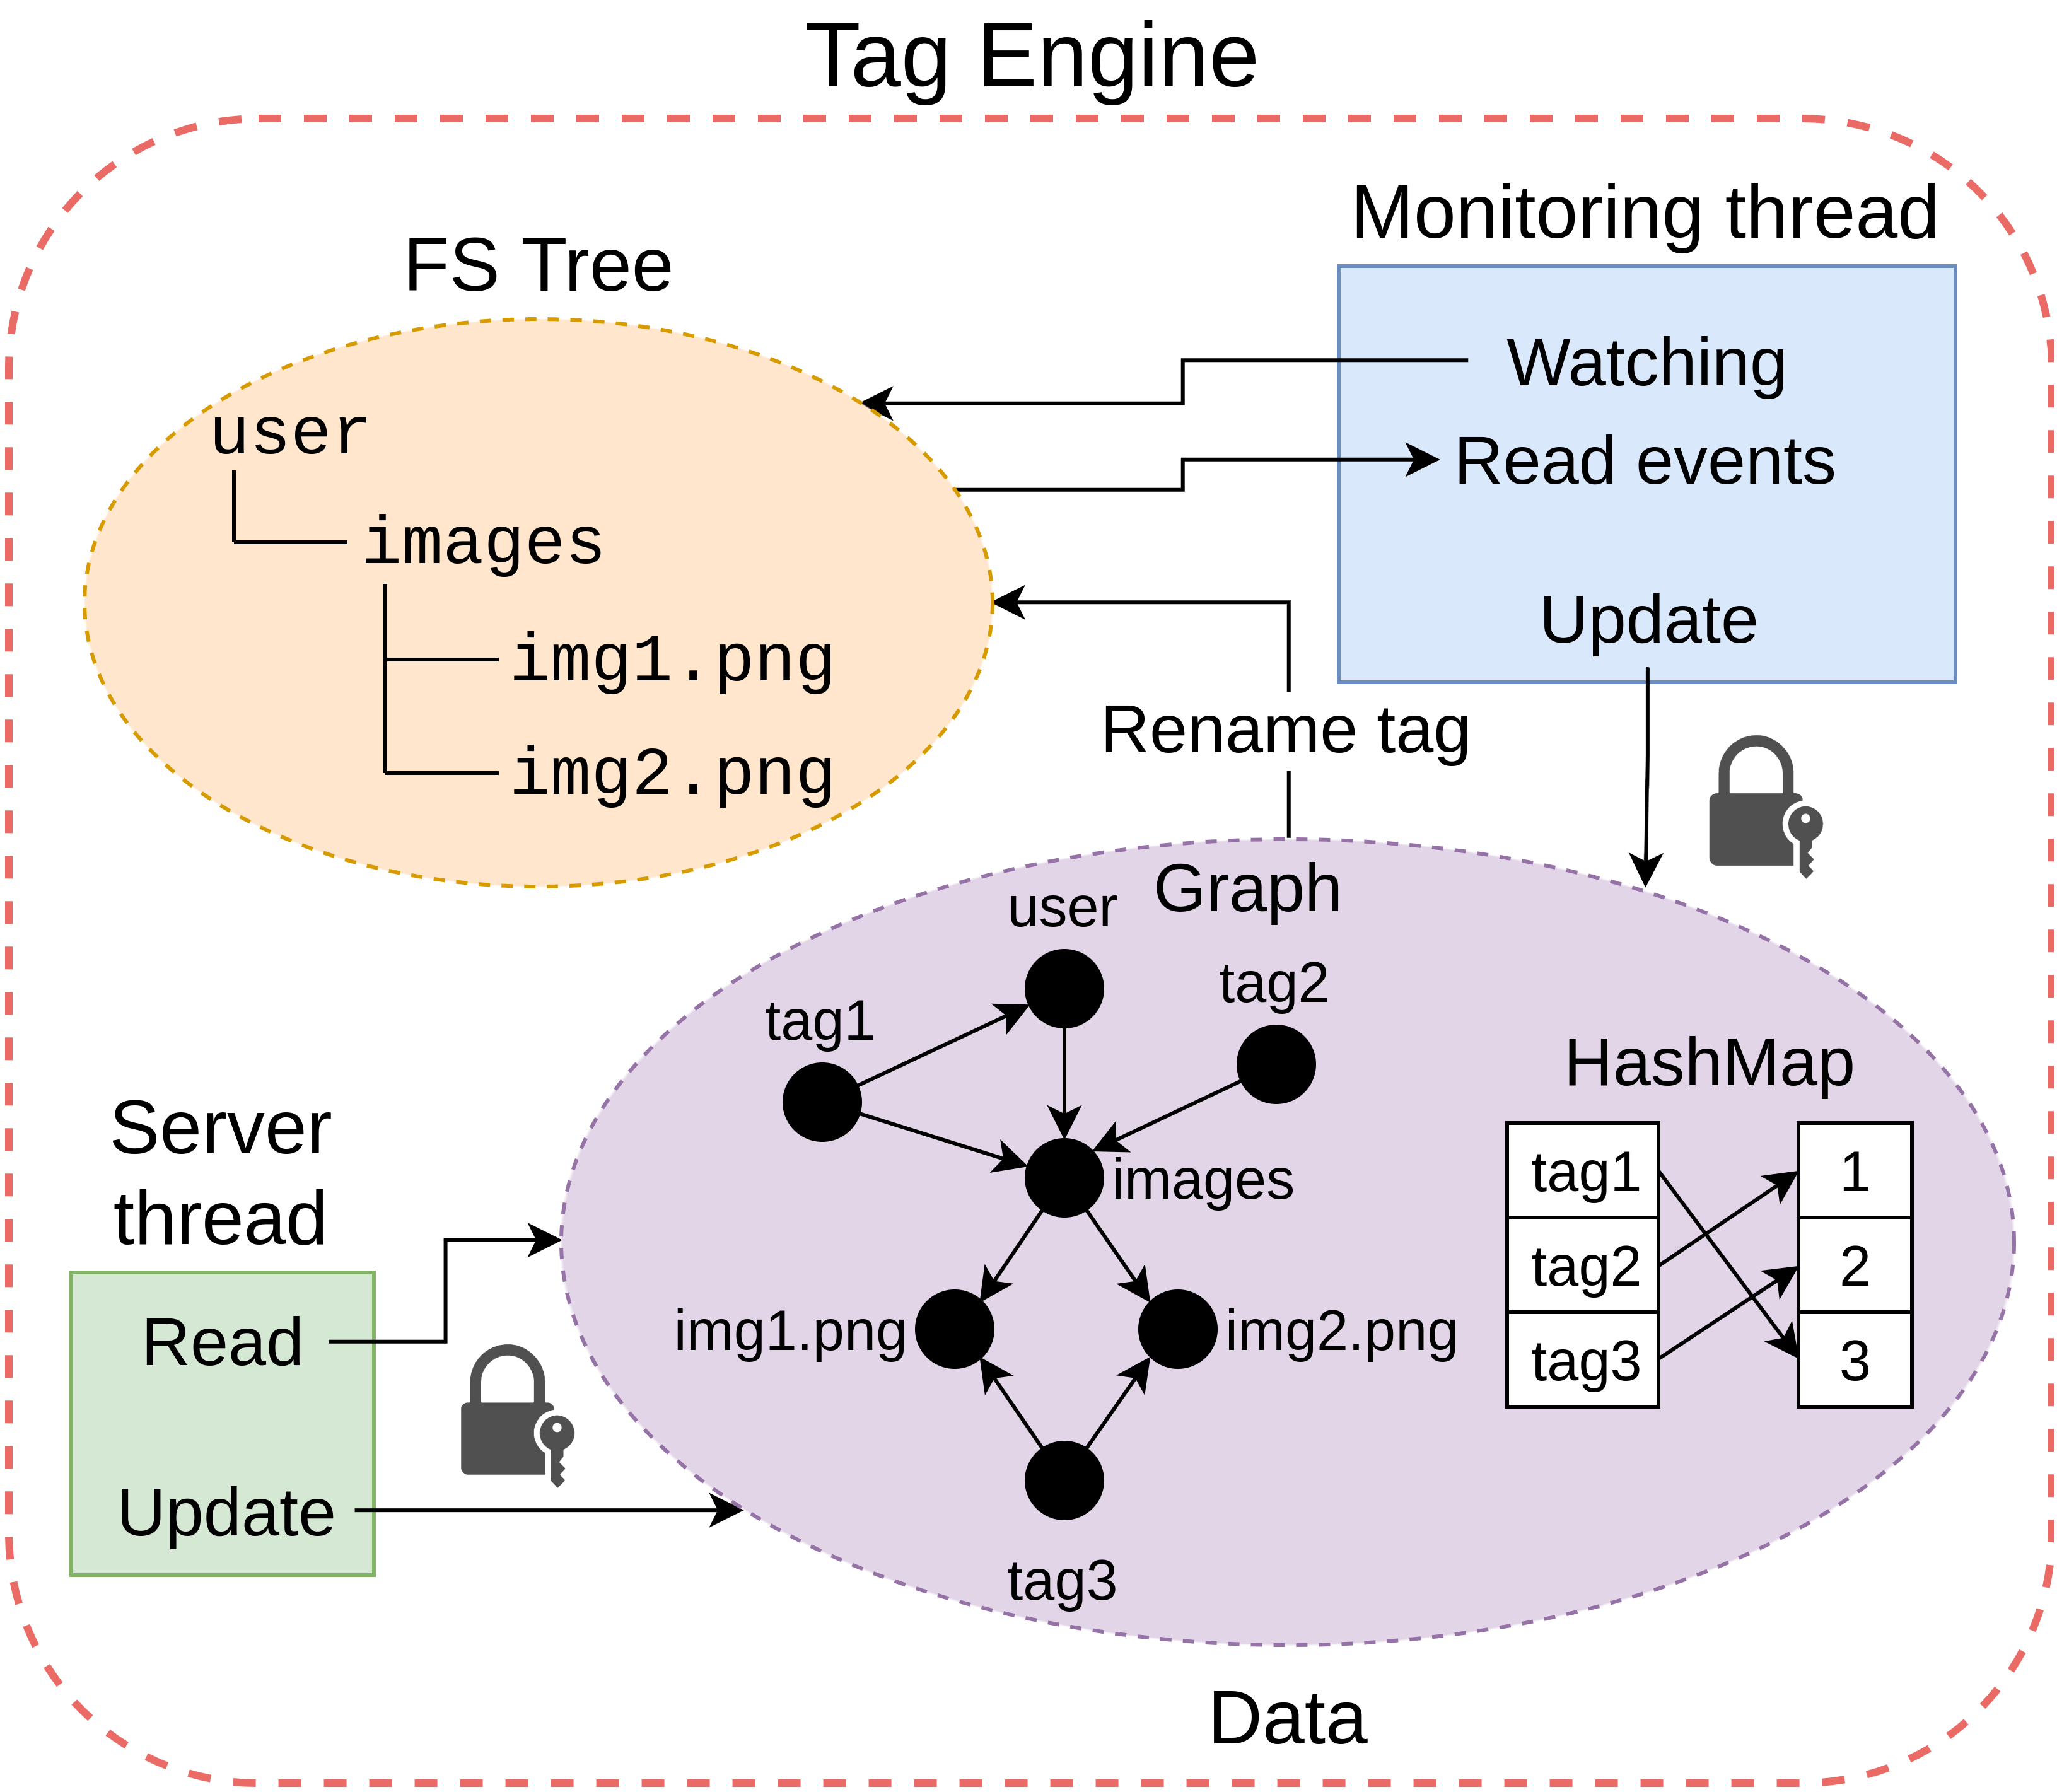
\includegraphics[width=0.7\textwidth]{images/tag_engine2.png}
            \caption{Fonctionnement de Tag Engine}
        \end{center}
    \end{figure}
\end{frame}

\subsection{TagFS}
\begin{frame}
    \frametitle{\subsecname}
    \begin{figure}
        \begin{center}
            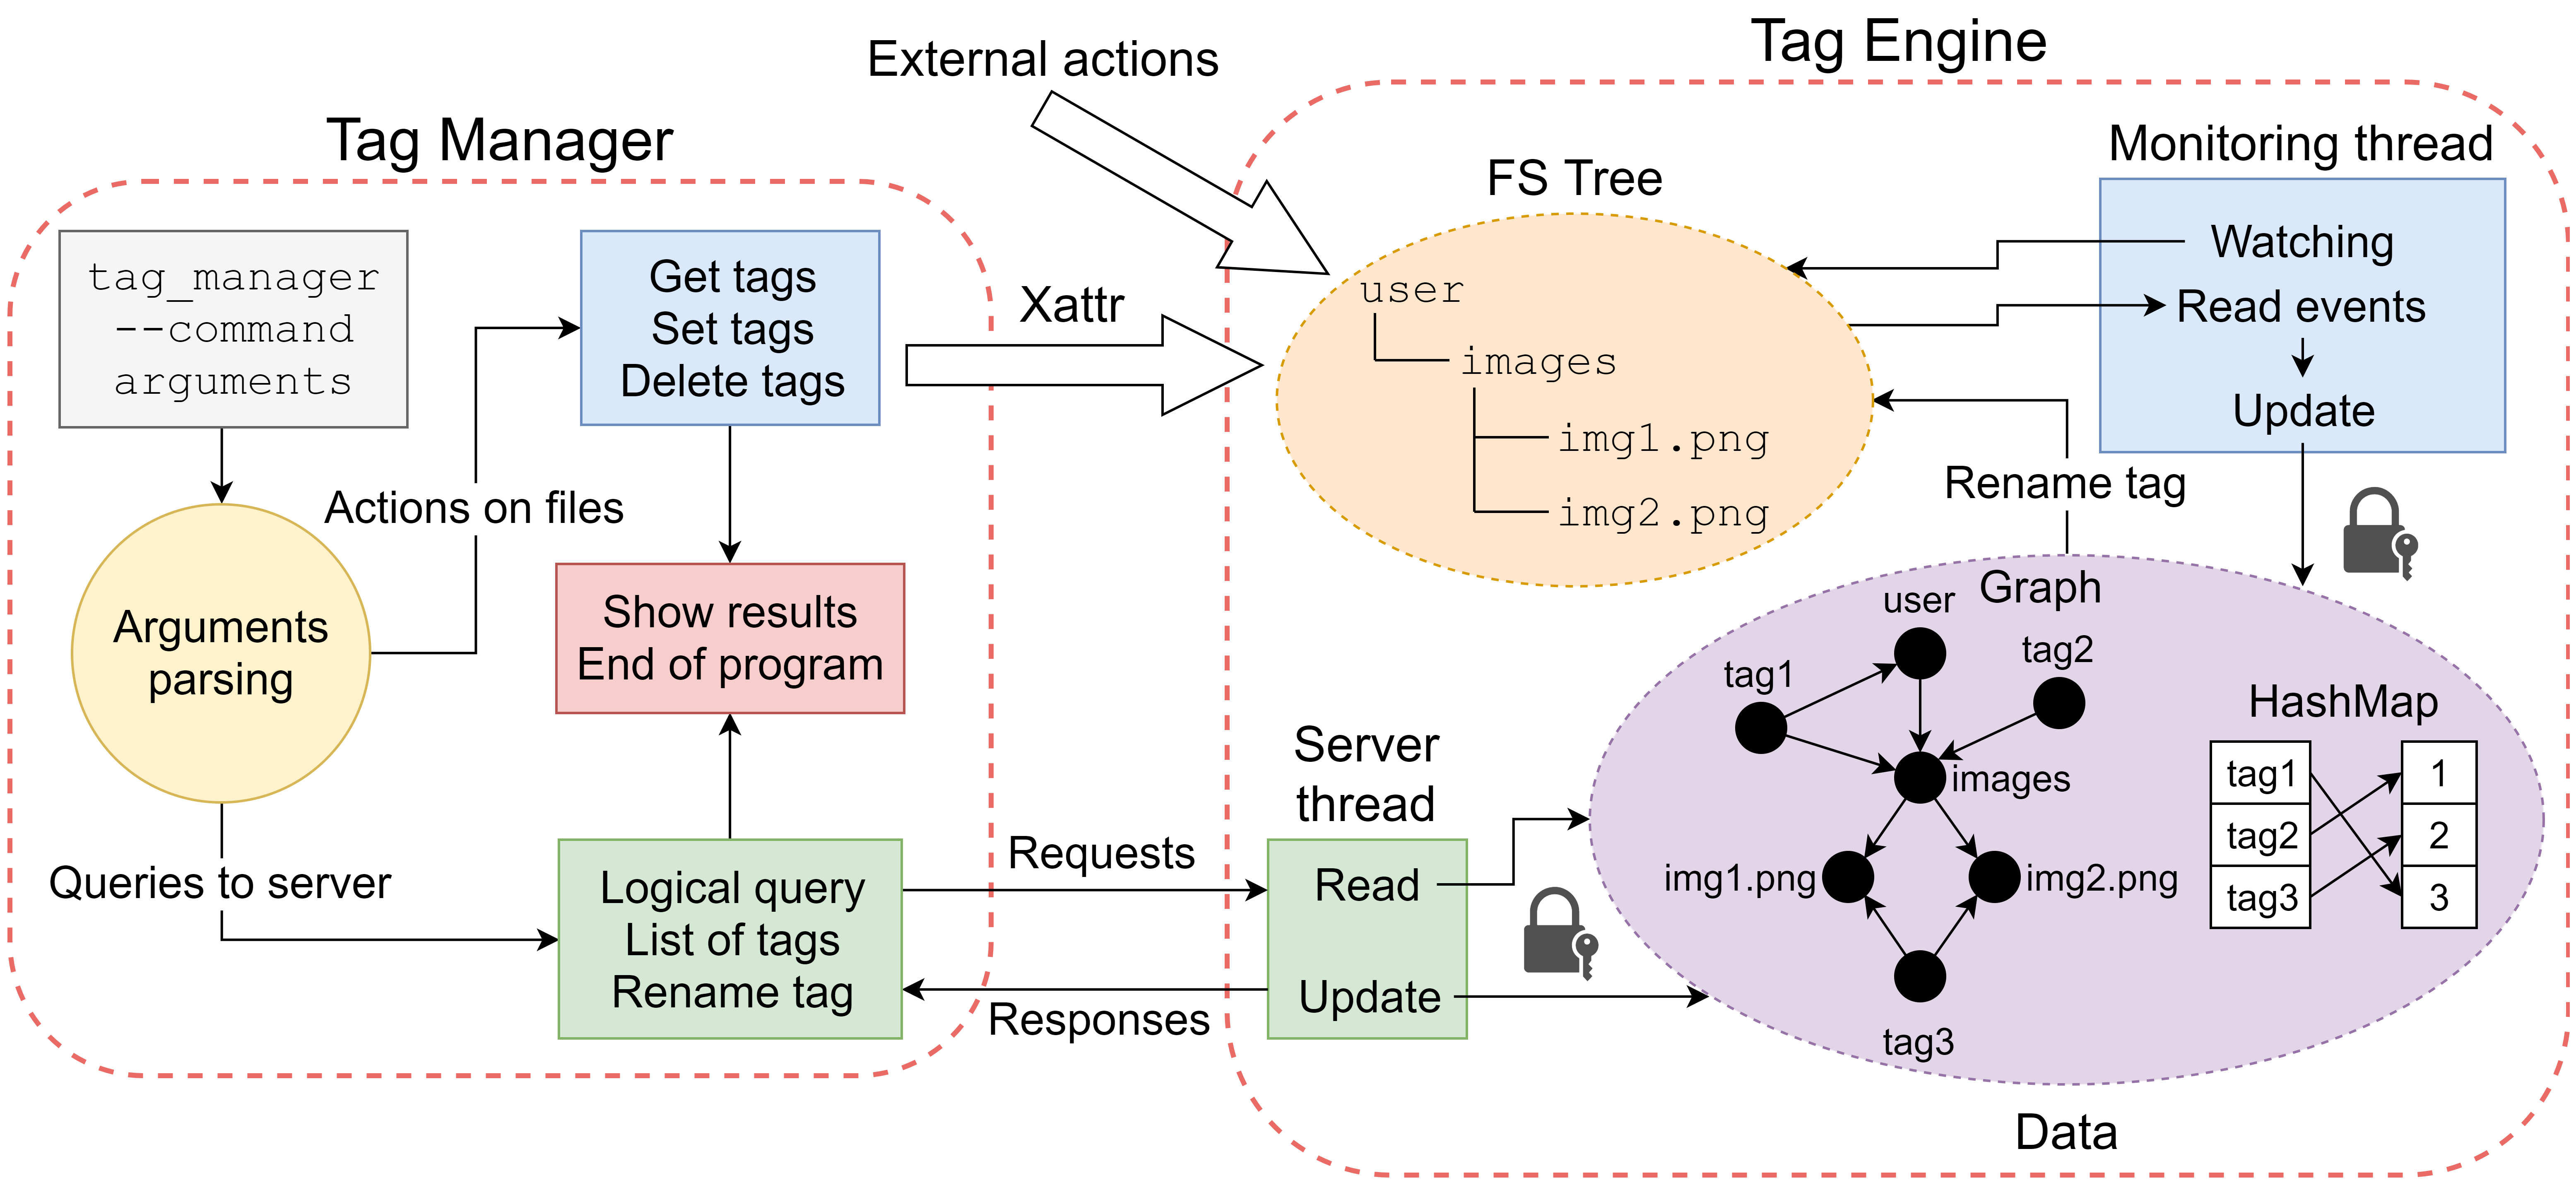
\includegraphics[width=1\textwidth]{images/tagfs4.png}
            \caption{Système global TagFS}
        \end{center}
    \end{figure}
\end{frame}

\subsection{Démo}
\begin{frame}
    \frametitle{\subsecname}
    \begin{center}
        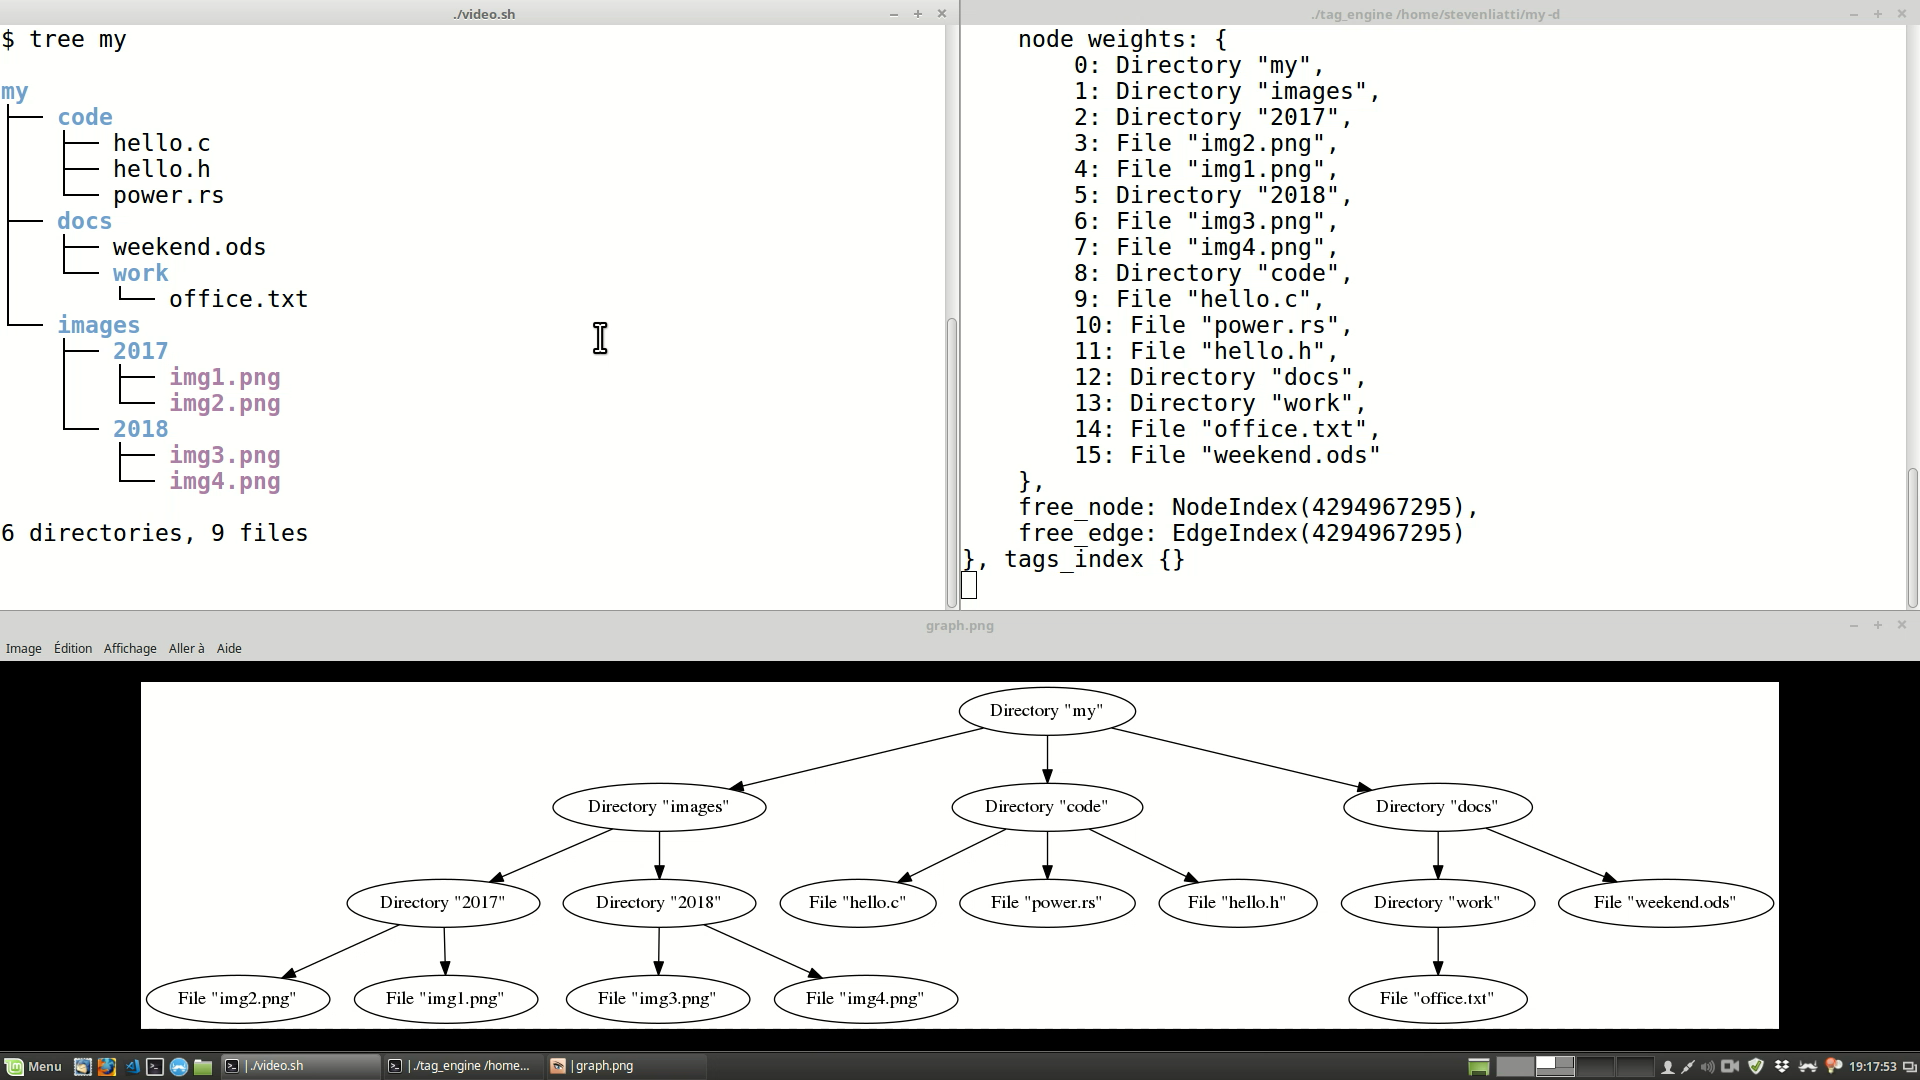
\includegraphics[width=0.8\textwidth]{images/video.png}
        \bigbreak
        \movie[externalviewer]{Vidéo}{video.mp4}
    \end{center}
\end{frame}

%%%%%%%%%%%%%%%%%%%%%%%%%%%%%%%%%%%%%%%%%%%%%%%%%%%%%%%%%%%%%%%%%%%%%%%%%%%%%%%%%%%%%%%%%%%%%%%%%%%
%%%%%%%%%%%%%%%%%%%%%%%%%%%%%%%%%%%%%%%%%%%%%%%%%%%%%%%%%%%%%%%%%%%%%%%%%%%%%%%%%%%%%%%%%%%%%%%%%%%
\section{Discussion}
\subsection{Mesures de performances}
\begin{frame}
    \frametitle{\subsecname}
    \begin{columns}[T]
        \begin{column}{.35\textwidth}
            \begin{figure}
                \begin{center}
                    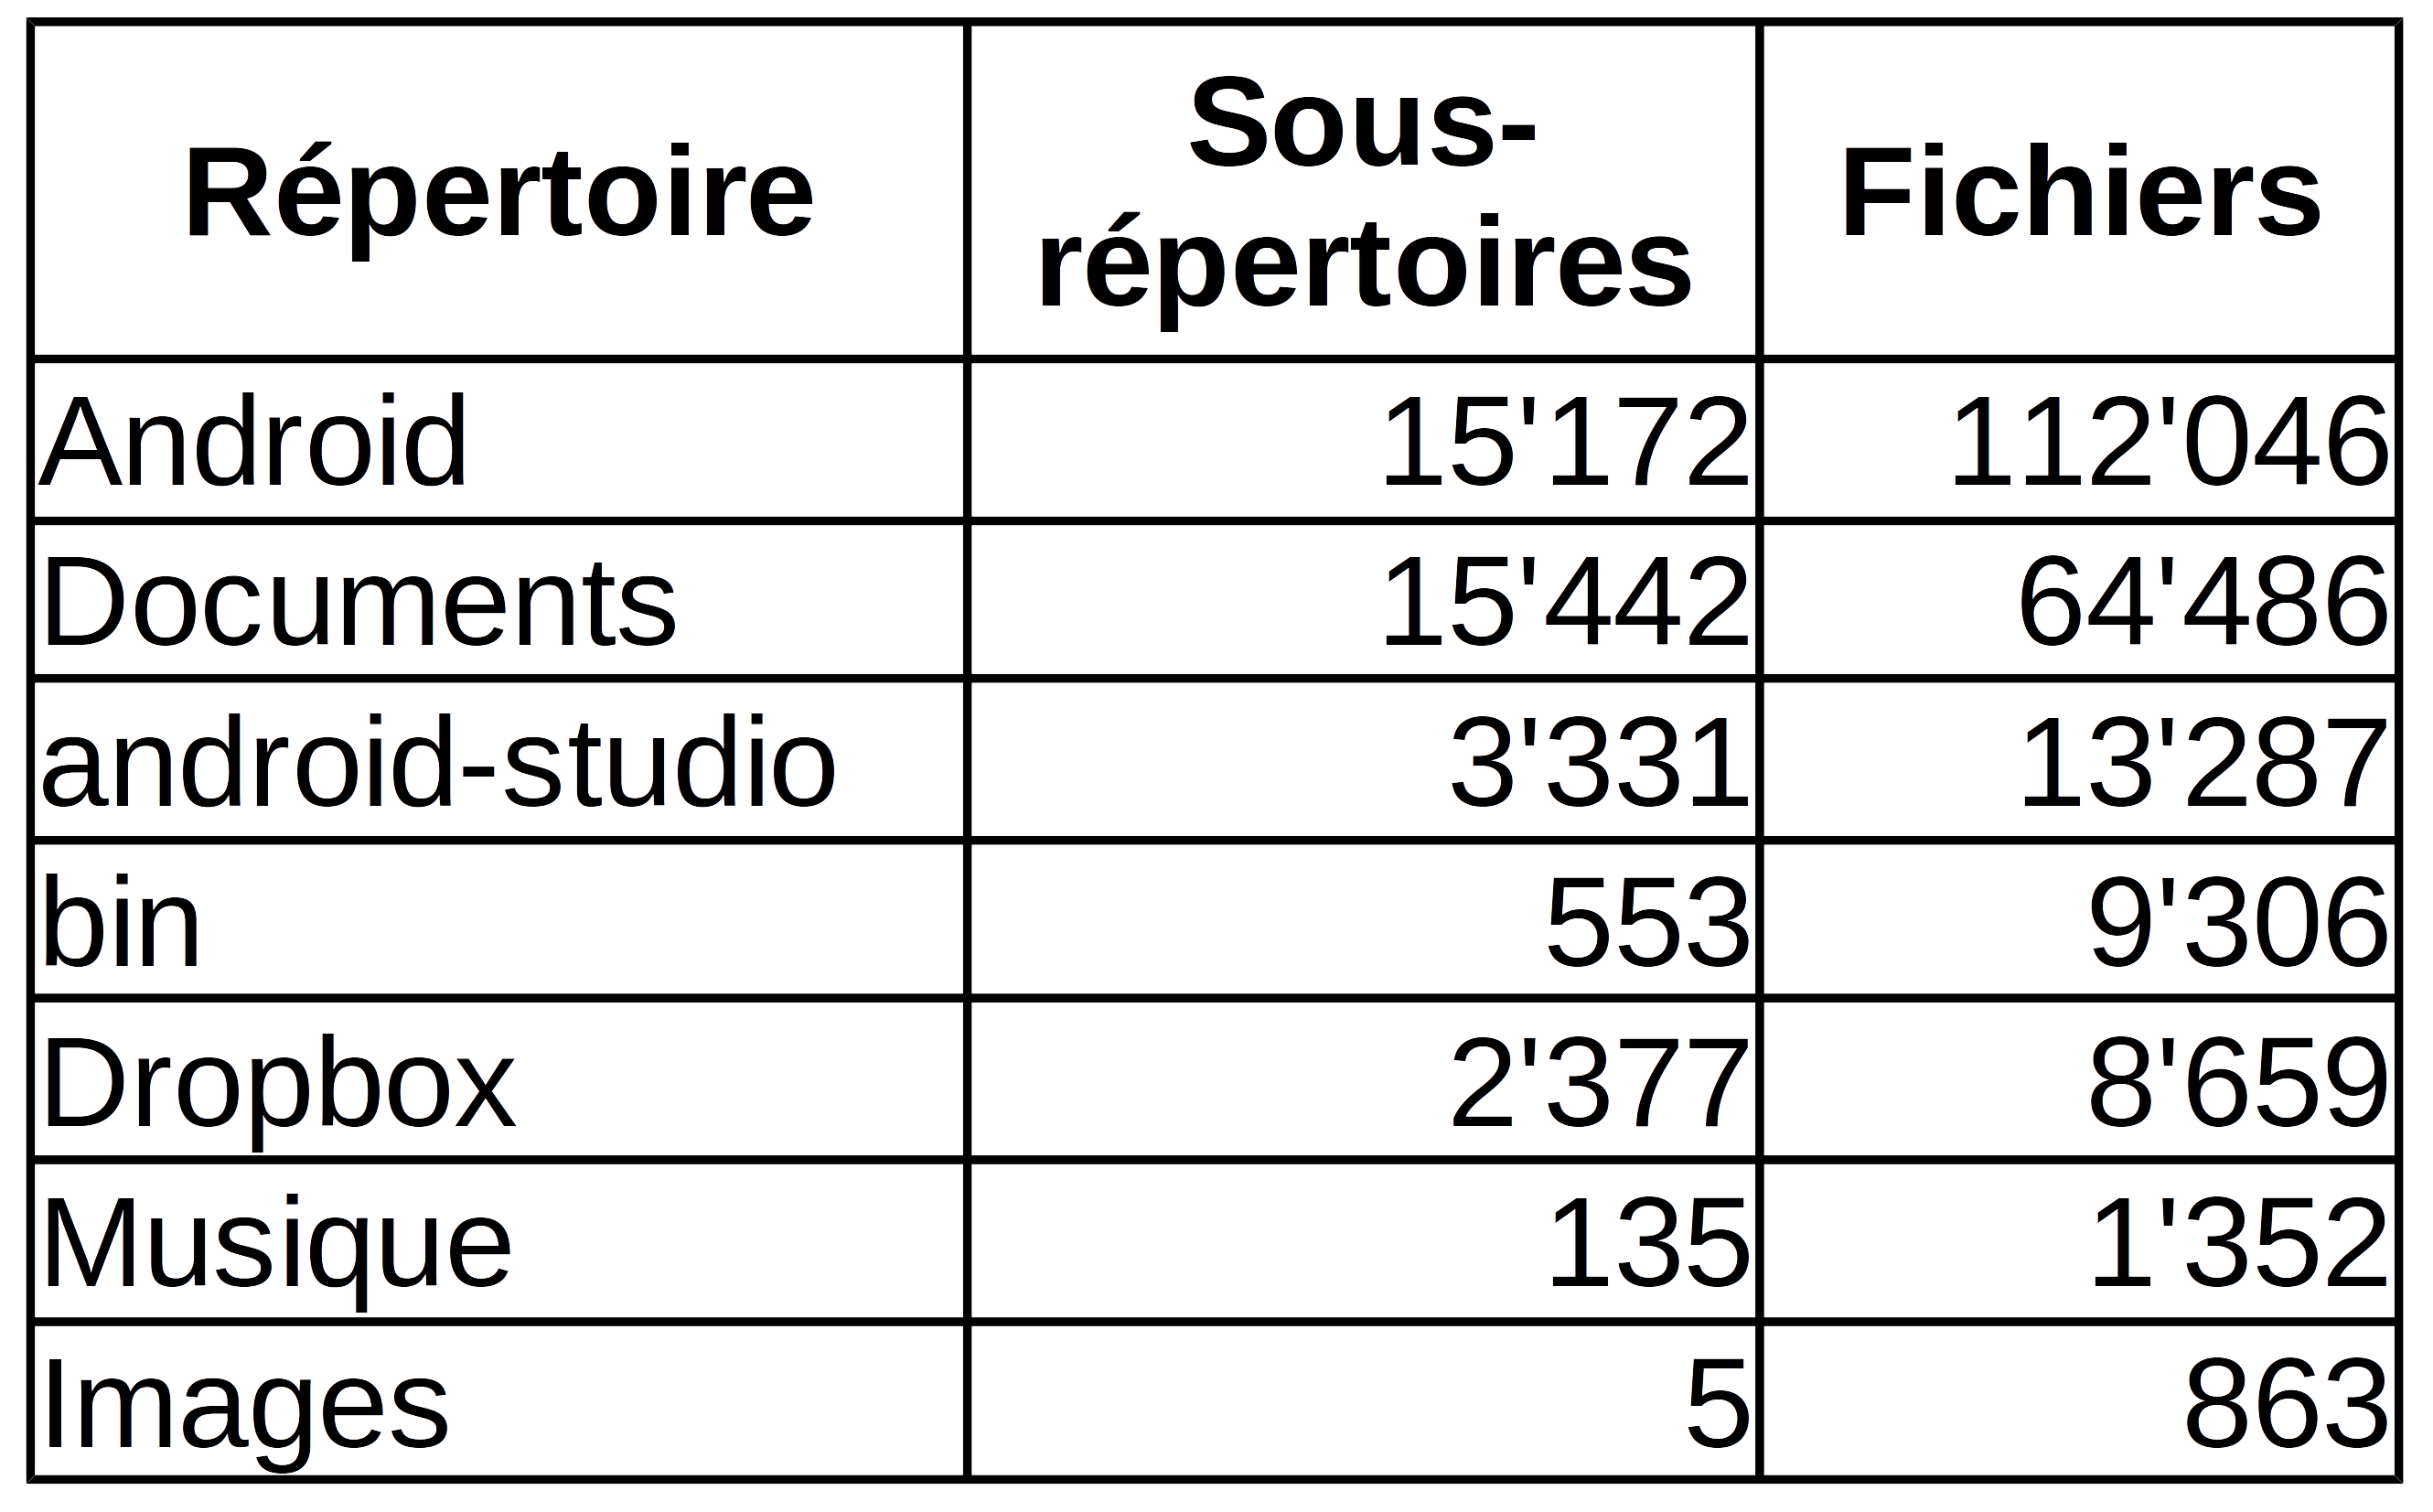
\includegraphics[width=1\textwidth]{images/tableau_rep.png}
                \end{center}
            \end{figure}
        \end{column}
        \begin{column}{.65\textwidth}
            \begin{figure}
                \begin{center}
                    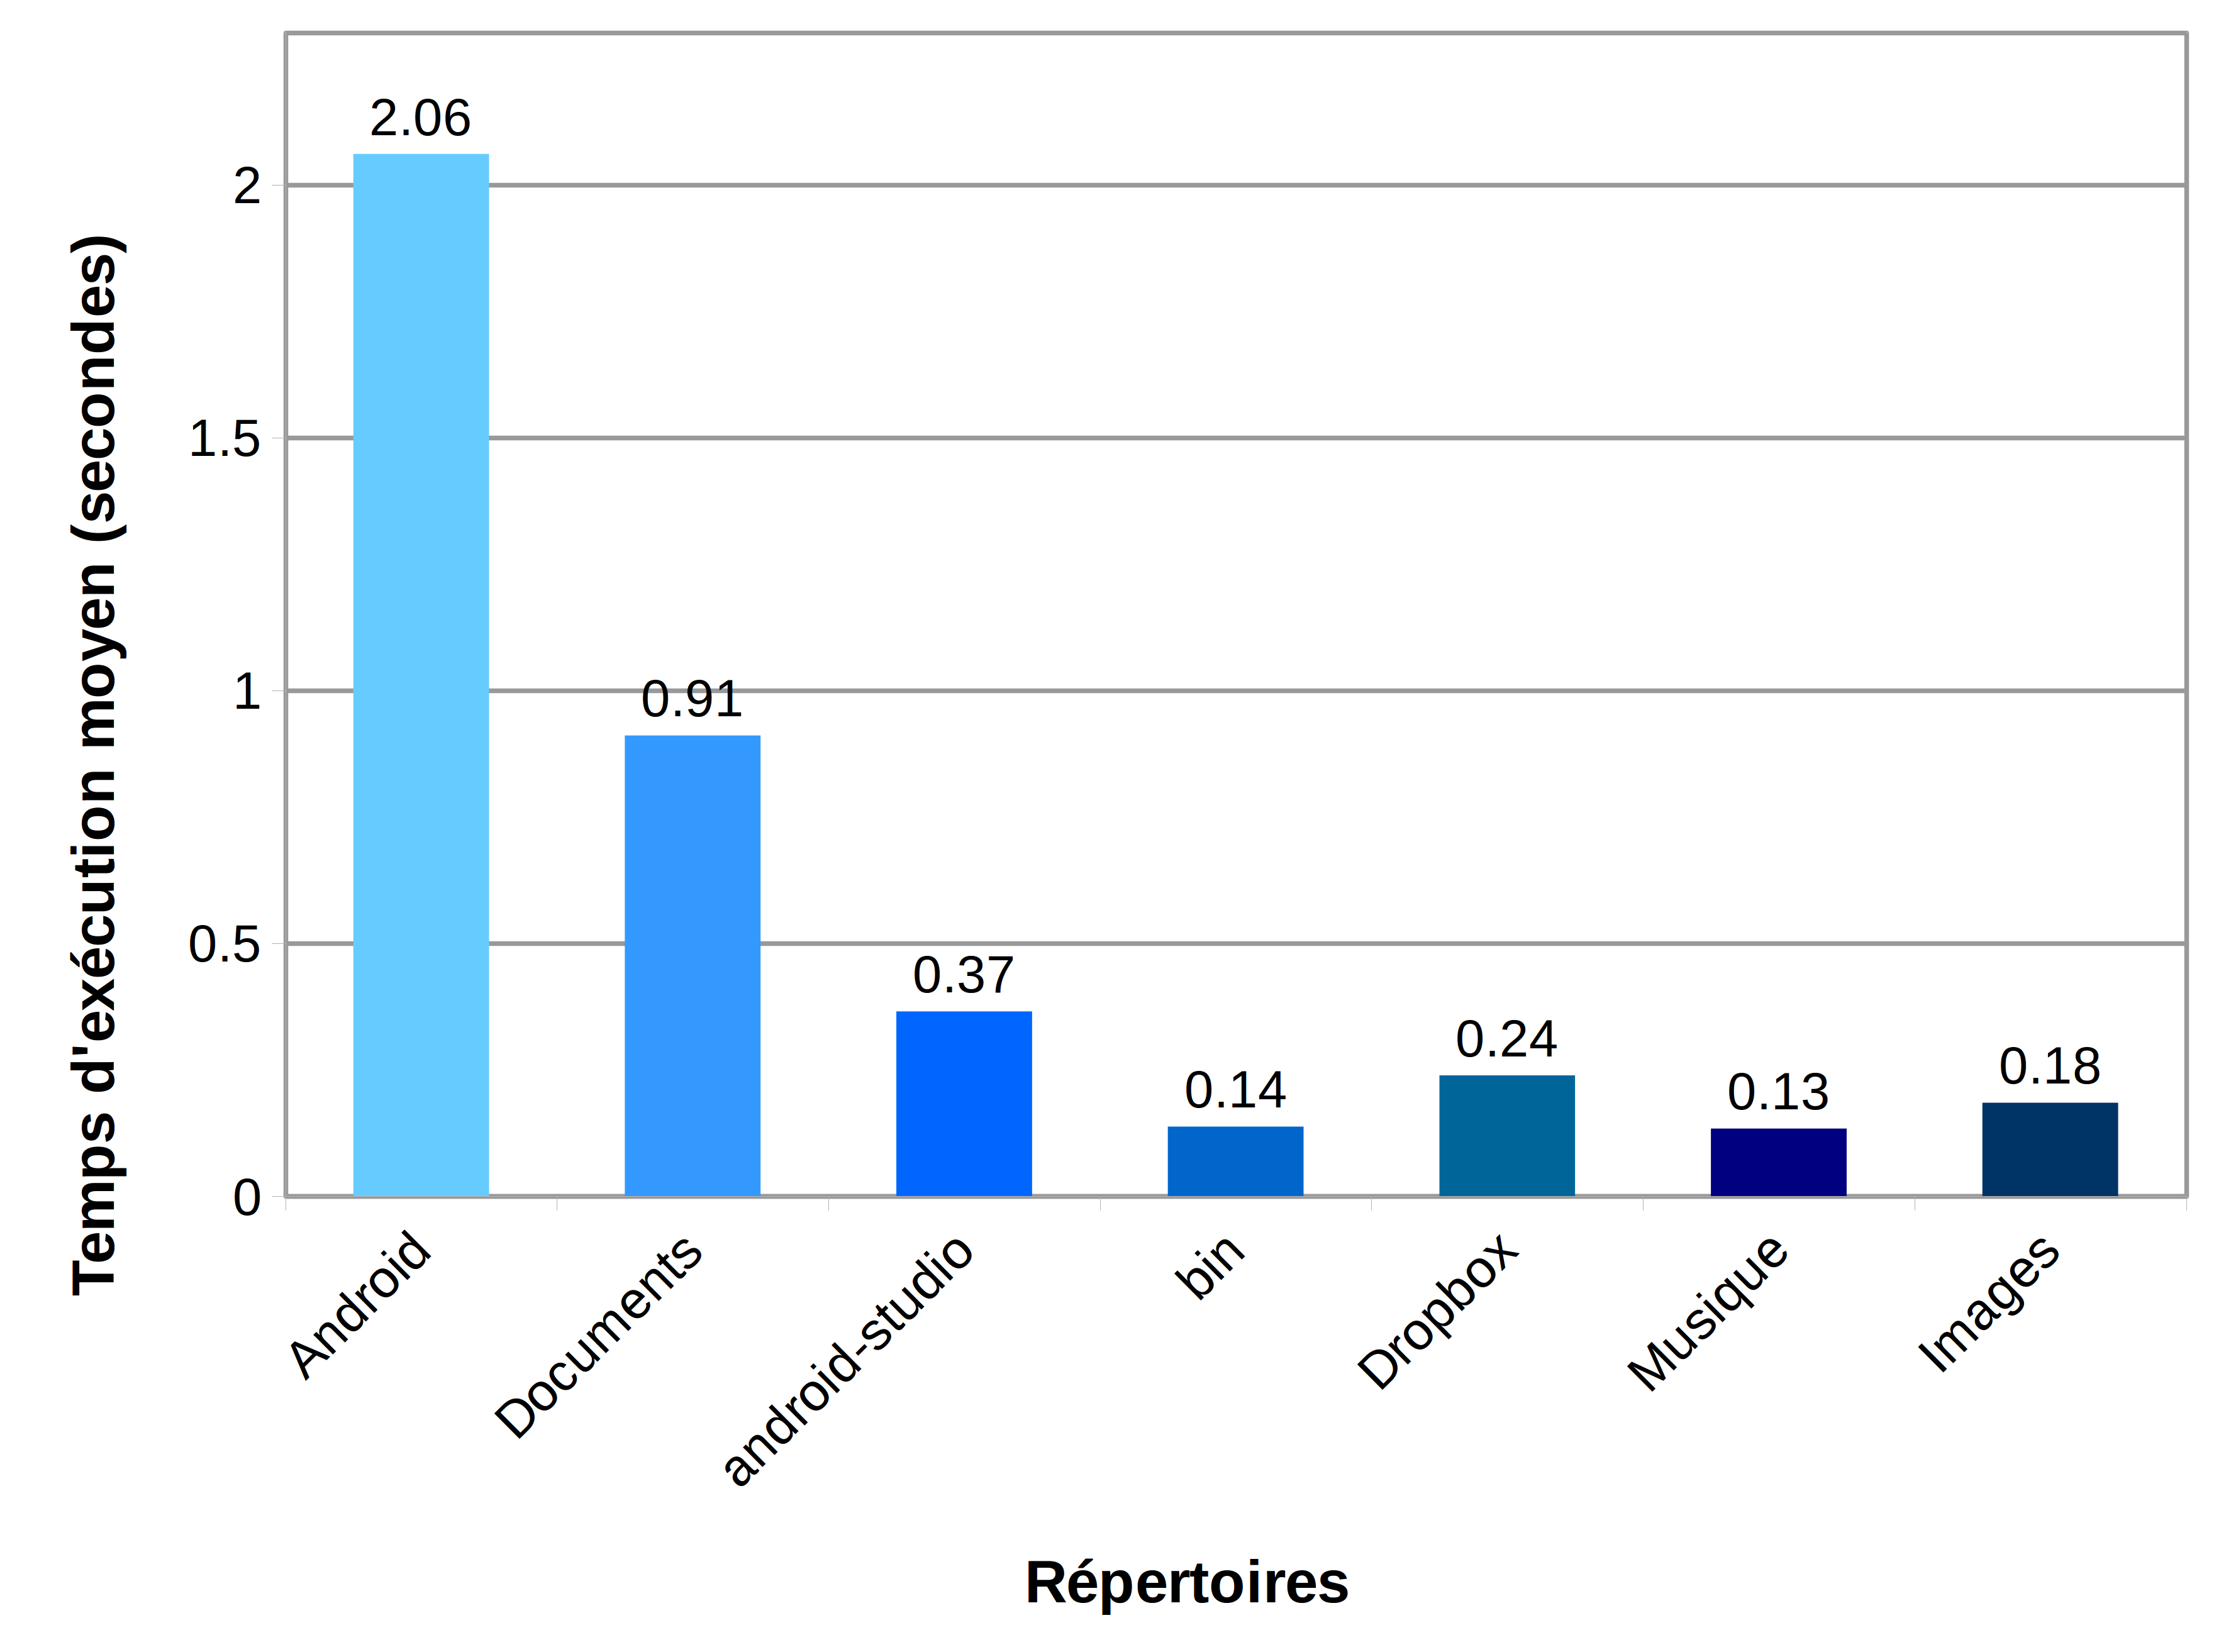
\includegraphics[width=1\textwidth]{images/histo4.png}
                    \caption{Temps d'exécution de Tag Engine en fonction des répertoires}
                \end{center}
            \end{figure}
        \end{column}
    \end{columns}
\end{frame}

%%%%%%%%%%%%%%%%%%%%%%%%%%%%%%%%%%%%%%%%%%%%%%%%%%%%%%%%%%%%%%%%%%%%%%%%%%%%%%%%%%%%%%%%%%%%%%%%%%%
%%%%%%%%%%%%%%%%%%%%%%%%%%%%%%%%%%%%%%%%%%%%%%%%%%%%%%%%%%%%%%%%%%%%%%%%%%%%%%%%%%%%%%%%%%%%%%%%%%%
\subsection{Améliorations}
\begin{frame}
    \frametitle{\subsecname}
    \begin{itemize}
        \pause
        \item GUI : environnement de bureau ou application web.
        \pause
        \item Daemon pour Tag Engine.
        \pause
        \item Ajout de nouveaux répertoires de surveillance (partiel).
        \pause
        \item Gestion des périphériques amovibles (limitation inotify).
        \pause
        \item Cache des dernières requêtes logiques adressées au serveur.
        \pause
        \item Ajouter des opérateurs logiques (NOT).
    \end{itemize}
\end{frame}

\section{Conclusion}
\subsection{Bilan personnel}
\begin{frame}
    \frametitle{\subsecname}
    \begin{itemize}
        \pause
        \item Conception d'un moteur de gestion de tags.
        \pause
        \item Étude du langage Rust.
        \pause
        \item Diverses technologies et approches.
        \pause
        \item \textbf{Progression personnelle : technologies, bonnes pratiques, démarche.}
    \end{itemize}
\end{frame}

%%%%%%%%%%%%%%%%%%%%%%%%%%%%%%%%%%%%%%%%%%%%%%%%%%%%%%%%%%%%%%%%%%%%%%%%%%%%%%%%%%%%%%%%%%%%%%%%%%%
%%%%%%%%%%%%%%%%%%%%%%%%%%%%%%%%%%%%%%%%%%%%%%%%%%%%%%%%%%%%%%%%%%%%%%%%%%%%%%%%%%%%%%%%%%%%%%%%%%%
\subsection{Remerciements}
\begin{frame}
    \frametitle{\subsecname}
    \begin{itemize}
        \item Florent Glück
        \item Orestis Malaspinas
        \item Joël Cavat
    \end{itemize}
    \bigbreak
    \pause
    \fontsize{14pt}{15}\selectfont
    \begin{center}
        \textbf{Merci pour votre attention ! Questions ?}
    \end{center}
\end{frame}


\end{document}
